\subsection*{Exercise 4}
\boldmath
\textbf{For any $0 \leq k \leq n$, the Johnson graph $J(n, k)$ is the graph defined as follows. The vertex set of
$J(n, k)$ consists of all $k$-elements subsets of $[n]$. Two vertices of $J(n, k)$ are adjacent if and only
if their intersection has size precisely $k-1$.} 
\begin{enumerate}[a)]
    \item \textbf{Draw $J(5, 3)$, clearly labelling all the vertices.} 
    \unboldmath
    \\
    \linebreak 
    The graph $J(5,3)$ has $\binom{n}{k}$ = $\binom{5}{3}$ = 10 vertices as follows: 
    \begin{multicols}{2}
    $v_1 = \{1, 2, 3\}$ \\
    $v_2 = \{1, 2, 4\}$ \\
    $v_3 = \{1, 2, 5\}$ \\
    $v_4 = \{1, 3, 4\}$ \\
    $v_5 = \{1, 3, 5\}$ \\
    $v_6 = \{1, 4, 5\}$ \\
    $v_7 = \{2, 3, 4\}$ \\
    $v_8 = \{2, 3, 5\}$ \\
    $v_9 = \{2, 4, 5\}$ \\
    $v_{10} = \{3, 4, 5\}$ 
    \end{multicols}
    In order for a pair of vertices $u$ and $v$ to be adjacent, the two vertices must have $k-1 = 2$ elements in common, i.e. $|u \cap v| = 2$. Hence, we obtain the following adjacency matrix:
    \[
\begin{blockarray}{ccccccccccc}
& v_1 & v_2 & v_3 & v_4 & v_5 & v_6 & v_7 & v_8 & v_9 & v_{10}\\
\begin{block}{c(cccccccccc)}
  v_1 & 0 & 1 & 1 & 1 & 1 & 0 & 1 & 1 & 0 & 0 \\
  v_2 & 1 & 0 & 1 & 1 & 0 & 1 & 1 & 0 & 1 & 0 \\
  v_3 & 1 & 1 & 0 & 0 & 1 & 1 & 0 & 1 & 1 & 0 \\
  v_4 & 1 & 1 & 0 & 0 & 1 & 1 & 1 & 0 & 0 & 1 \\
  v_5 & 1 & 0 & 1 & 1 & 0 & 1 & 0 & 1 & 0 & 1 \\
  v_6 & 0 & 1 & 1 & 1 & 1 & 0 & 0 & 0 & 1 & 1 \\
  v_7 & 1 & 1 & 0 & 1 & 0 & 0 & 0 & 1 & 1 & 1 \\
  v_8 & 1 & 0 & 1 & 0 & 1 & 0 & 1 & 0 & 1 & 1 \\
  v_9 & 0 & 1 & 1 & 0 & 0 & 1 & 1 & 1 & 0 & 1 \\
  v_{10} & 0 & 0 & 0 & 1 & 1 & 1 & 1 & 1 & 1 & 0 \\
\end{block}
\end{blockarray}
 \]
This results in the graph $G$, where $|V| = 10$ and $|E| = 30$ : \\
\begin{center}
    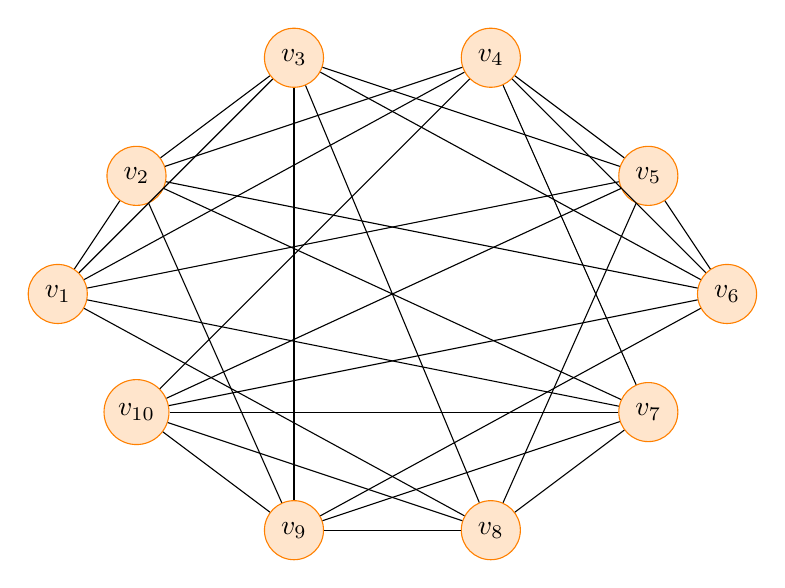
\begin{tikzpicture}
    \tikzset{
    dep/.style={circle,minimum size=0.75cm,fill=orange!20,draw=orange},
    c1/.style={-},
    c2/.style={dotted, red, line width=2},
    }
    \node[dep] (n1) at (0,0) {$v_1$};
    \node[dep] (n2) at (1,1.5) {$v_2$};
    \node[dep] (n3) at (3,3) {$v_3$}; 
    \node[dep] (n4) at (5.5,3) {$v_4$};
    \node[dep] (n5) at (7.5,1.5) {$v_5$};
    \node[dep] (n6) at (8.5,0) {$v_6$};
    \node[dep] (n7) at (7.5,-1.5) {$v_7$};
    \node[dep] (n8) at (5.5,-3) {$v_8$};
    \node[dep] (n9) at (3,-3) {$v_9$};
    \node[dep] (n10) at (1,-1.5) {$v_{10}$};
    
    \draw[c1] (n1) edge node[above] {} (n2);
    \draw[c1] (n1) edge node[above] {} (n3);
    \draw[c1] (n1) edge node[above] {} (n4);
    \draw[c1] (n1) edge node[above] {} (n5);
    \draw[c1] (n1) edge node[above] {} (n7);
    \draw[c1] (n1) edge node[above] {} (n8);
    
    \draw[c1] (n2) edge node[above] {} (n3);
    \draw[c1] (n2) edge node[above] {} (n4);
    \draw[c1] (n2) edge node[above] {} (n6);
    \draw[c1] (n2) edge node[above] {} (n7);
    \draw[c1] (n2) edge node[above] {} (n9);

    \draw[c1] (n3) edge node[above] {} (n5);
    \draw[c1] (n3) edge node[above] {} (n6);
    \draw[c1] (n3) edge node[above] {} (n8);
    \draw[c1] (n3) edge node[above] {} (n9);

    \draw[c1] (n4) edge node[above] {} (n5);
    \draw[c1] (n4) edge node[above] {} (n6);
    \draw[c1] (n4) edge node[above] {} (n7);
    \draw[c1] (n4) edge node[above] {} (n10);

    \draw[c1] (n5) edge node[above] {} (n6);
    \draw[c1] (n5) edge node[above] {} (n8);
    \draw[c1] (n5) edge node[above] {} (n10);

    \draw[c1] (n6) edge node[above] {} (n9);
    \draw[c1] (n6) edge node[above] {} (n10);

    \draw[c1] (n7) edge node[above] {} (n8);
    \draw[c1] (n7) edge node[above] {} (n9);
    \draw[c1] (n7) edge node[above] {} (n10);

    \draw[c1] (n8) edge node[above] {} (n9);
    \draw[c1] (n8) edge node[above] {} (n10);
    
    \draw[c1] (n9) edge node[above] {} (n10);
    
\end{tikzpicture}   
\end{center} 
    \boldmath
    \item \textbf{Show that $J(n, k)$ and $J(n, n-k)$ are isomorphic for any $0 \leq k \leq n.$} \\\linebreak 
    \unboldmath
    \boldmath
    \item \textbf{Determine the average degree, number of edges, diameter, and girth of $J(n, k)$ for each $0 \leq k \leq n$.} \\\linebreak
    \unboldmath
\end{enumerate}
